\documentclass[11pt]{article}

\usepackage{amsmath}
\usepackage{amsfonts}
\usepackage[margin=1in]{geometry}
\usepackage{enumitem}
\usepackage{graphicx}
\usepackage[colorlinks]{hyperref}
\usepackage{longtable}

\usepackage{helvet}
\renewcommand{\familydefault}{\sfdefault}

\setlength{\parindent}{0in}

\def\tightlist{}
\def\toprule{}
\def\bottomrule{}

\begin{document}
{\LARGE Homework 10 (Due December
2nd)}\label{homework-10-due-december-2nd}

{\Large 1. Ampere's Law}\label{amperes-law}

Consider a thick SLAB of current.

\begin{figure}[htbp]
\centering
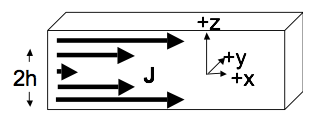
\includegraphics[width=0.6\linewidth]{./images/hw10/thick_slab.png}
\end{figure}

The slab is infinite in (both) \(x\) and \(y\), but finite in \(z\). So
we must think about the volume current density \(\mathbf{J}\), rather
than \(\mathbf{K}\). The slab has thickness \(2h\) (It runs from
\(z=-h\) to \(z=+h\)) Let's assume that the current is still flowing in
the \(+x\) direction, and is uniform in the \(x\) and \(y\) dimensions,
but now \(\mathbf{J}\) depends on height linearly, i.e.
\(\mathbf{J} = J_0\,\mathrm{abs}(z)\,\hat{x}\), inside the slab (but is
0 above or below the slab), where \(\mathrm{abs}(z)\) is the absolute
value of \(z\).

\begin{enumerate}
\def\labelenumi{\arabic{enumi}.}
\tightlist
\item
  Find the B field (magnitude and direction) everywhere in space (above,
  below, and also, most interestingly, inside the slab!)
\end{enumerate}

{\Large 2. Quick Ampere's Law}\label{quick-amperes-law}

Suppose \(\mathbf{B}\) in a region of space centered on the origin has
cylindrical symmetry and is given by \(\mathbf{B} = B_0\hat{\phi}\)
where \(B_0\) is a constant, and \(\hat{phi}\) is the azimuthal
direction in cylindrical coordinates.

\begin{enumerate}
\def\labelenumi{\arabic{enumi}.}
\tightlist
\item
  What is the current density in this region of space?
\item
  Suppose the current density that you found extends out to a radius
  \(R\) and is zero for \(r > R\). What is the magnetic field for
  \(r > R\)?
\end{enumerate}

{\Large 3. Ampere and superposition}\label{ampere-and-superposition}

A clever use of superposition should can make seemingly complicated
situations easier to solve.

\begin{figure}[htbp]
\centering
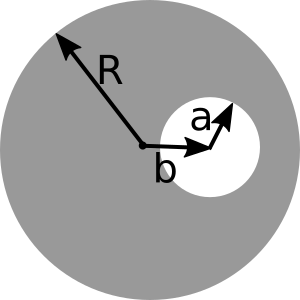
\includegraphics[width=0.4\linewidth]{./images/hw10/wire_w_hole.png}
\end{figure}

\begin{enumerate}
\def\labelenumi{\arabic{enumi}.}
\tightlist
\item
  A long (infinite) wire (cylindrical conductor of radius \(R\), whose
  axis coincides with the \(z\) axis) carries a uniformly distributed
  current \(I_0\) in the \(+z\) direction. A cylindrical hole is drilled
  out of the conductor, parallel to the \(z\) axis, (see figure above
  for geometry). The center of the hole is at \(x = b\), and the radius
  is \(a\). Determine the magnetic field \emph{in the hole region.}
\item
  If this is an ordinary wire carrying ordinary household currents, and
  the drilled hole has dimensions roughly shown to scale in the figure
  above, make an order of magnitude estimate for the strength of the
  \(B\) field in that region. How does it compare to the earth's field?
  \emph{You should find that the B field in the hole is uniform - that
  was just a little surprising to me!}
\end{enumerate}

{\Large 4. Formal manipulations and vector
calculus}\label{formal-manipulations-and-vector-calculus}

Griffiths (section 5.3.2) shows that, given Biot-Savart, we can arrive
at Ampere's law.

\begin{enumerate}
\def\labelenumi{\arabic{enumi}.}
\item
  Go through that derivation and try to recreate it/make sense of it.
  \textbf{Don't just copy it down - do all the steps yourself.} There
  are a few ``gaps'' in his derivation that you should be explicit about
  - e.g., Eq 5.50 (.52 in the 4th ed) is missing terms, what happened to
  them? Are you convinced of the minus sign shenanigans leading to 5.52
  (.54 in 4th ed)? Convince us you understand them! Do you understand
  the ending: why did the contribution in Eq. 5.53 (.55 in 4th ed) ``go
  away''?
\item
  Use similar mathematical gymnastics to start from the Biot-Savart law
  and end with \(\mathbf{B} = \nabla \times \mathbf{A}\), where
  \(\mathbf{A}(\mathbf{r}) = \dfrac{\mu_0}{4 \pi} \int \dfrac{\mathbf{J}(\mathbf{r}')}{\mathfrak{R}}d\tau'\).
  (this is Griffiths Eq 5.63, or .65 in 4th edition). You'll do this in
  a different way than Griffiths does (though I suggest you convince
  yourself you can see it his way too, which is section 5.4.1!). (Note:
  Part 2 is easier than part 1, really!!)
\end{enumerate}

\begin{itemize}
\tightlist
\item
  Start with the Biot-Savart law (Eq 5.45 , or 5.47 in the 4th ed).
\item
  Make use of the handy identity we've seen several times this term:
  \(\nabla \dfrac{1}{\mathfrak{R}} = -\dfrac{1}{\mathfrak{R}^2}\hat{\mathfrak{R}}\)
  (Do you know where this relation comes from, can you show it?)\\
\item
  Then use Griffiths' product rule \#7 (front flyleaf) to manipulate
  your expression until you get to . That ``something'' should be
  precisely the formula we're after!\\
  \emph{At some point you will need to pull the curl past an integral
  sign - be sure to justify why this is a perfectly legitimate thing to
  do.}
\end{itemize}

{\Large 5. Fields and Strengths}\label{fields-and-strengths}

\begin{enumerate}
\def\labelenumi{\arabic{enumi}.}
\tightlist
\item
  Estimate the density \(\rho\) of mobile charges in a piece of
  gold-wire speaker wire, assuming each atom contributes one free
  electron. (Look up any necessary physical constants!) Then, think
  about the definition of current, and \emph{estimate} the average
  electron speed in a gold speaker wire of ordinary household size
  carrying an ordinary household current. Your answer will come out
  quite slow - it might surprise you. If you flip on the stereo, and the
  speakers are, say, 2 meters away, would there be a noticeable ``time
  lag'' before you hear the speaker come on?
\item
  If you cut open this wire, you'll see it is really two wires, each
  insulated, and wrapped close together in a single plastic cylinder
  (since you need a complete circuit, current has to flow TO and FROM
  the speaker, right?). Make reasonable guesses for the dimensions
  involved in a real, ordinary speaker wire, to estimate the TOTAL
  magnetic force between the ``outgoing'' and ``return'' wires. Is it
  attractive or repulsive? Now - if you could somehow remove the
  stationary positive ions in the metallic conductor (which play no role
  in the flow of current, right?), make a rough estimate for the total
  electrical force of repulsion between the two wires. How does it
  compare with the magnetic force you just found?
\end{enumerate}

{\Large 6. Vector Potential I}\label{vector-potential-i}

\begin{enumerate}
\def\labelenumi{\arabic{enumi}.}
\tightlist
\item
  A long (infinite) wire (cylindrical conductor, radius \(R\), whose
  axis coincides with the \(z\) axis) carries a uniformly distributed
  current \(I_0\) in the \(+z\) direction. Assuming
  \(\nabla \cdot \mathbf{A} = 0\) (the ``Coulomb gauge''), and choosing
  \(\mathbf{A}=0\) at the edge of the wire, show that the vector
  potential inside the wire could be given by \(A= c I_0(1-s^2/R^2)\).
  Find the constant \(c\) (including units.) Things to explicitly
  find/discuss: What is the vector direction of \(\mathbf{A}\)? (Does it
  ``make sense'' in any way to you?) Is your answer unique, or is there
  any remaining ``ambiguity'' in \(\mathbf{A}\)? (Note that we're not
  asking you to derive \(\mathbf{A}\) from scratch, just to see that
  this choice of A ``works'')
\item
  What is the vector potential outside that wire? (Make sure that it
  still satisfies \(\nabla \cdot \mathbf{A} = 0\), and make sure that
  \(\mathbf{A}\) is continuous at the edge of the wire, consistent with
  part 1). Here again, is your answer unique, or is there any remaining
  ``ambiguity'' in \(\mathbf{A}(outside)\)?
\end{enumerate}

{\Large 7. Vector Potential II}\label{vector-potential-ii}

Griffiths Fig 5.48 is a handy ``triangle'' summarizing the mathematical
connections between \(\mathbf{J}\), \(\mathbf{A}\), and \(\mathbf{B}\)
(like Fig. 2.35) But there's a missing link, he has nothing for the left
arrow from \(\mathbf{B}\) to \(\mathbf{A}\). Note the equations defining
\(\mathbf{A}\) are very analogous to the basic Maxwell's equations for
\(\mathbf{B}\):

\[\nabla \cdot \mathbf{B} = 0 \leftrightarrow \nabla \cdot \mathbf{A} = 0\]

\[\nabla \times \mathbf{B} = \mu_0\mathbf{J} \leftrightarrow \nabla \times \mathbf{A} = \mathbf{B}\]

\begin{enumerate}
\def\labelenumi{\arabic{enumi}.}
\item
  So \(\mathbf{A}\) depends on \(\mathbf{B}\) in the same way
  (mathematically) the \(\mathbf{B}\) depends on \(\mathbf{J}\). (Think,
  Biot-Savart!) Use this idea to just write down a formula for
  \(\mathbf{A}\) in terms of \(\mathbf{B}\) to finish off that triangle.
\item
  In lecture notes (and/or Griffiths Ex. 5.9) we found the
  \(\mathbf{B}\) field everywhere inside (and outside) an infinite
  solenoid (which you can think of as a cylinder with uniform surface
  current flowing azimuthally around it (see figure below). See Griff.
  Fig 5.35. Use the basic idea from the previous part of this question
  to, therefore, quickly and easily just write down the vector potential
  \(\mathbf{A}\) in a situation where \(\mathbf{B}\) looks analogous to
  that, i.e. \(\mathbf{B} = C\delta(s-R)\hat{\phi}\), with \(C\)
  constant. Also, sketch this \(\mathbf{A}\) for us, please. (You should
  be able to just ``see'' the answer, no nasty integral needed!)\\
\item
  For you to discuss: What physical situation creates such a
  \(\mathbf{B}\) field? (This is tricky - think about it!) Also, if I
  gave you some \(\mathbf{B}\) field and asked for \(\mathbf{A}\), can
  you now think of an ``analogue method'', i.e.~an experiment where you
  could let nature do this for you, instead of computing it? \emph{It's
  cool - think about what's going on here. You have a previously solved
  problem, where a given \(\mathbf{J}\) led us to some \(\mathbf{B}\).
  Now we immediately know what the vector potential is in a very
  different physical situation, one where \(\mathbf{B}\) happens to look
  like \(\mathbf{J}\) did in that previous problem.}
\end{enumerate}

\begin{figure}[htbp]
\centering
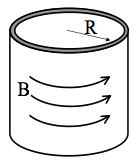
\includegraphics[width=0.3\linewidth]{./images/hw10/b_circulate.png}
\end{figure}
\end{document}
